The organization of the architecture is described in Figure \ref{fig:gra}.

First a module User Interface will be used by the user to play the game. Then the User Interface will transmit the data to the module Model. The model is able to make the move, to update the board. If the game is a human game, the Model will only interact with the User Interface. Otherwise, for the computer move, it will communicate with the MCTS module via the API. This API is here to make communicate the Model and the MCTS module. The MCTS is using an implementation of the parallelization to compute his algorithm faster, using different computers.

\begin{figure}[!h]
\centering
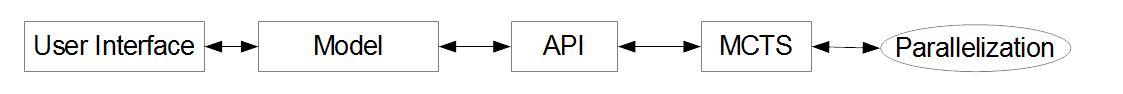
\includegraphics[width=1\textwidth]{2General_Architecture/2.1.2GeneralView/graphe2.png}
\caption{General view of the architecture}
\label{fig:gra}
\end{figure}


Here is a diagram showing the links between the interface and the rest of the modules in Figure \ref{fig:gen}

\begin{figure}[!h]
\centering
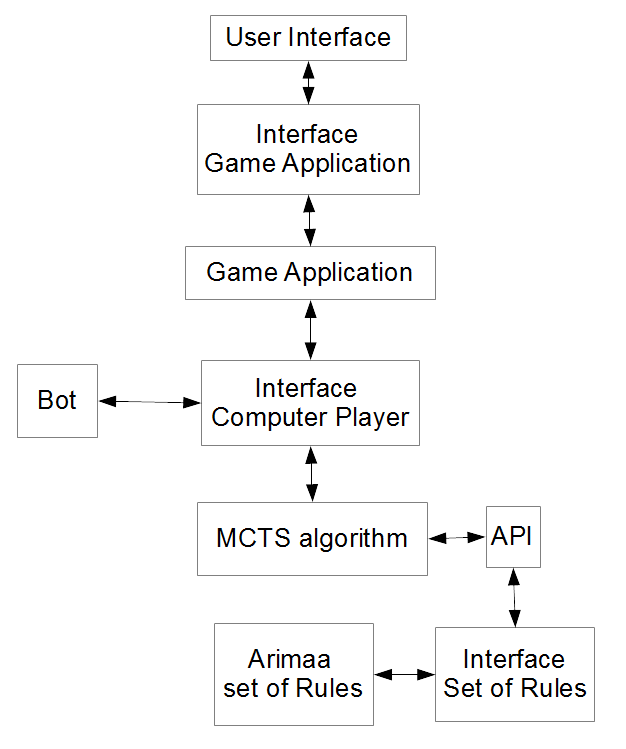
\includegraphics[width=0.5\textwidth]{2General_Architecture/2.1.2GeneralView/gen.png}
\caption{Interfaces of the architecture}
\label{fig:gen}
\end{figure}

The user will interact with the user interface, which will communicate with the game application, where all data for the game will be stored. Then, it will communicate with an Interface which will handle the communications between the Game application and the computer player. 

In our case, the computer player will be played by the AI using the MCTS algorithm, communicating with the Arimaa set of rules via the API and an interface for the set of Rules.  If another algorithm is to be tested, it will be added.

Interfaces are very important because they make it possible for others to use our project for others games than Arimaa without rebuilding everything. They would only have to implement the Interface with their proper game, game rules.

Furthermore, if the time permits it, the management of computers bots\footnote{For instance of the site \textit{Arimaa.com}} will be added. The only problem here is the computers bots are not similar to each other, thus it will take time to implement a class which will be able to communicate with both the computer bot and the interface.

The input of our software will be provided by the user using the mouse and keyboard. The output will only be the display of the screen, after the computer player makes a move.